\documentclass{article}%
\usepackage[T1]{fontenc}%
\usepackage[utf8]{inputenc}%
\usepackage{lmodern}%
\usepackage{textcomp}%
\usepackage{lastpage}%
\usepackage{geometry}%
\usepackage{float}%
\usepackage{biblatex}%
\usepackage{hyperref}%
\usepackage{subcaption}%
\usepackage{epigraph}

\addbibresource{citations.bib}
\geometry{tmargin=1cm,lmargin=0.75cm,rmargin=0.75cm}%
\usepackage{graphicx}%
\setlength{\parskip}{0.2em}%
%
\title{Experimental verification of the Faraday effect and estimation of the Verdet constant, V, across wavelengths.}%
\author{Brian Rogers}
\date{}%
%
\begin{document}%
\maketitle
\section*{Abstract}
In this report, I aim to provide experimental verification for the Faraday effect using F2 Schott glass under the influence of a magnetic field.
Further, I extend my investigation into the wavelength dependency of the Magneto-Optical effect and I measure the Verdet constants, V for a range of wavelengths in the visible spectrum. 


\section{Introduction}
\subsection{Historical background}
On the $30^{th}$ September 1845, Michael Faraday wrote in his daily notebook:

\textit{
"Still, I have at last succeeded in illuminating a magnetic curve or line of force, and in magnetizing a ray of light."
} 
\cite{Faraday}

By passing light through a piece of "heavy" glass he was able to observe that the plane of polarisation of light was rotated when an external magnetic field was applied. 
Finding other materials that displayed the same effect, he confirmed that the angle of rotation
was proportional to the magnetic field he applied to the material. Investigating the effect of a magnetised material on a path of light was a novel procedure as only certain materials had shown this property previously without magnetisation, as shown by Fresnel. \cite{Fresnel} 



\subsection{Theoretical background}

The Faraday effect can be summarised with the following equation 

\begin{equation}
    \Theta = V B L
\end{equation}

were $\Theta$ is the angle of rotation of the plane of linearly polarised light, $B$ is the applied magnetic field, $L$ is the length of the material used and V is the Verdet constant that depends on the material in question.

$\Theta$ can be given as 

\begin{equation}
    \Theta = \frac{\omega (n_{+} - n_{-})}{2c} B
\end{equation}
with $n_{+} - n_{-}$ being the respective refractive indices along different directions of the material induced by the applied magnetic field.
This difference in refractive indicies is the reason for rotation of the angle of polarisation.
In general, the Verdet constant can be written in terms of the incident wavelength, $\lambda$ as

\begin{equation}
    V = \frac{e\lambda}{2mc^{2}} \frac{\delta n}{\delta \lambda}
\end{equation}

Combining these equations we can generate a relation between the wavelength of incident radiation and the Verdet constant as 

\begin{equation}
    V = \frac{e\lambda}{2mc^{2}} \frac{1.8 \times 10^{-14}}{\lambda^{2}}
\end{equation}

The constant of proportionality included in the equation is given by the manufacturer's manual with no relevant uncertainity provided. \cite{Lab}
\section{Methods}

\subsection{Experimental}
\begin{figure}[H]%
    \centering%
    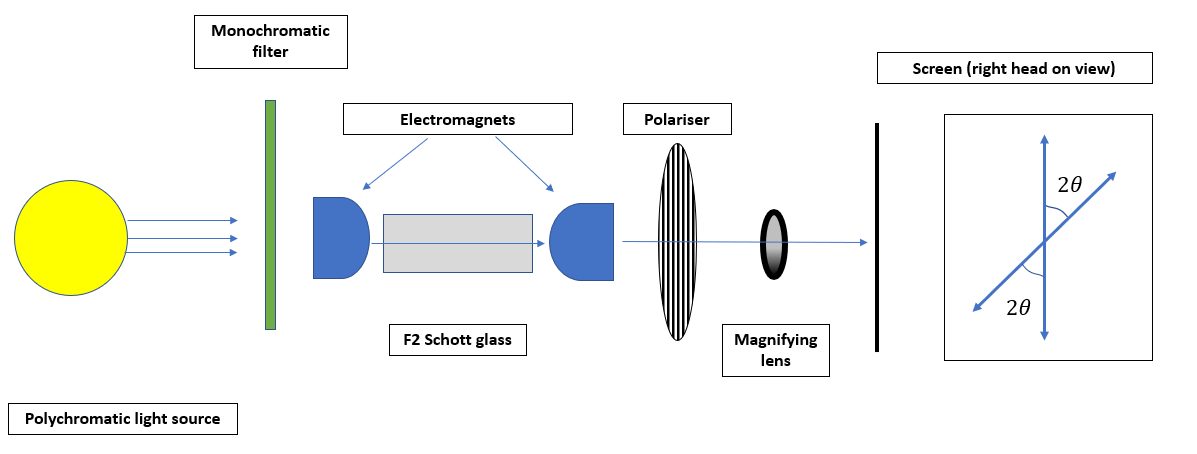
\includegraphics[width=500px]{setup.png}%
    \caption{Simplified experimental setup highlighting the key componets.}%
\end{figure}

Figure 1 shows the key operable components used in this experiment. A polychromatic source using a halogen lamp is incident upon a filter. This filter can be swapped to control the wavelength that reaches the F2 Schott glass. I made use of four separate filters. 
The glass itself is sandwiched between a pair of electromagnets. By varying the current through the electromagnets, I generated various field strengths in the region of the glass. Measurements of the field strengths as a function of input currents were taken with a Hall probe in place of the glass. The results are shown in figure 2 below.

\begin{figure}[H]%
    \centering%
    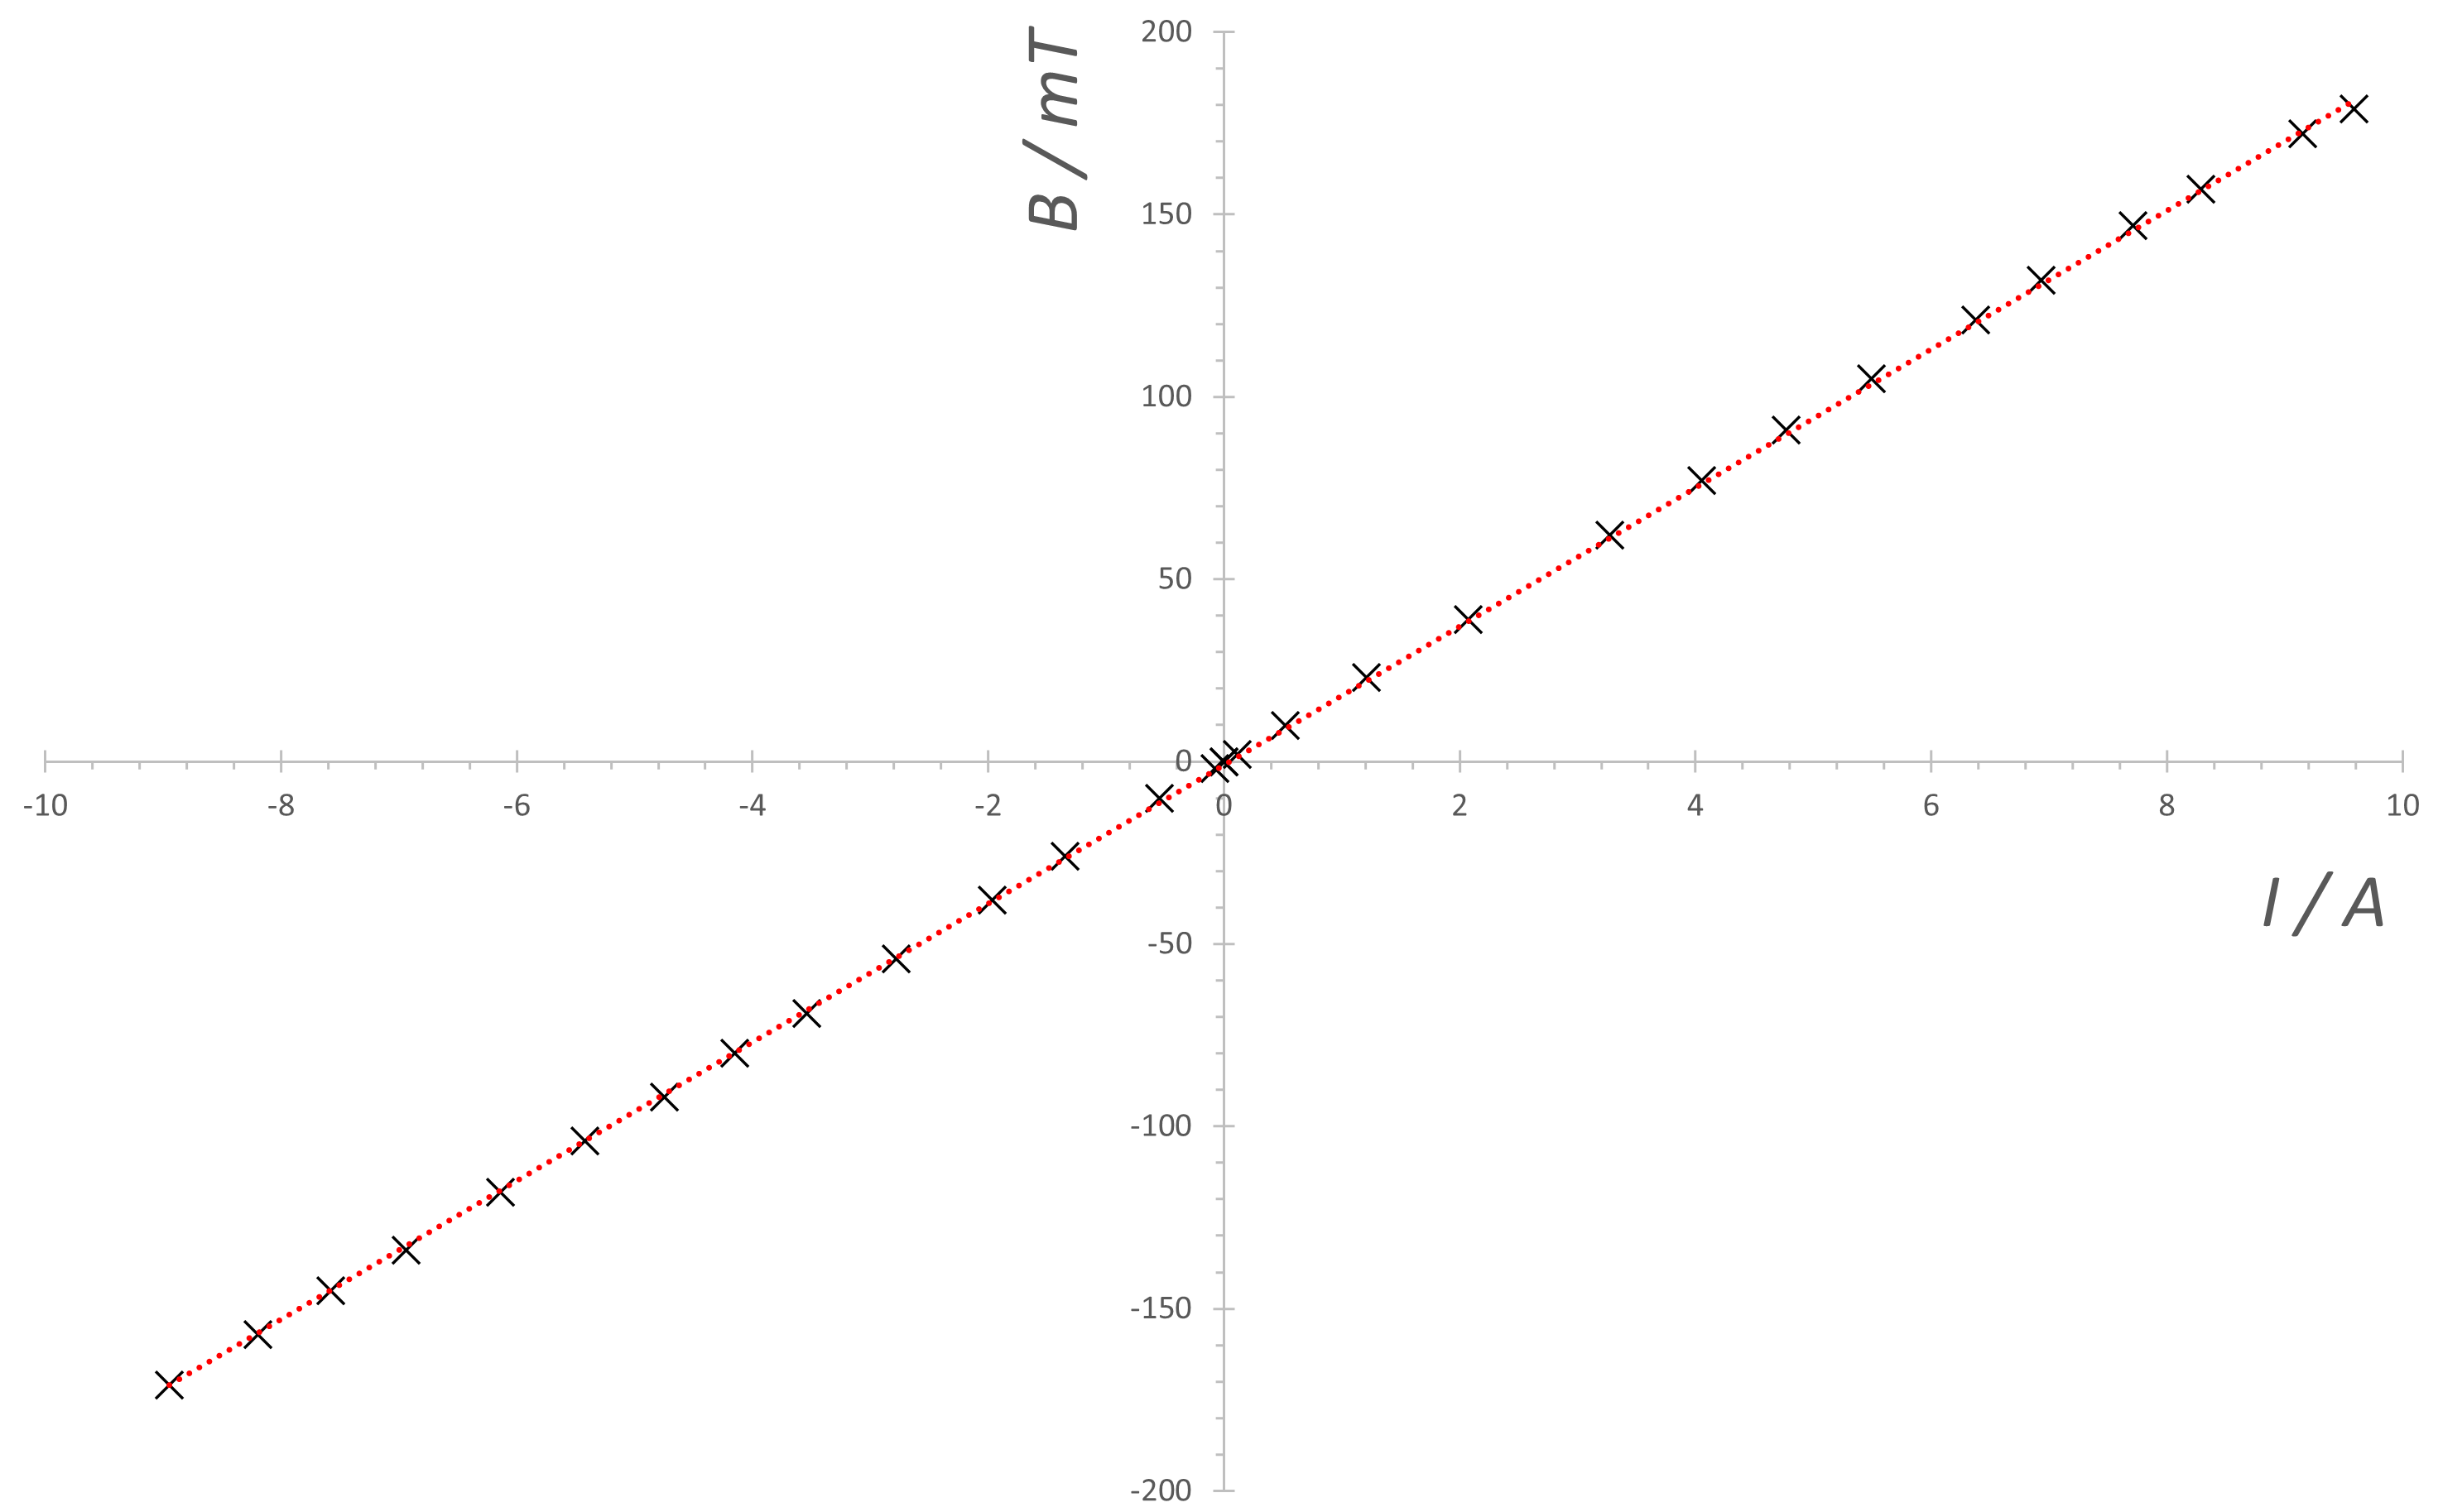
\includegraphics[width=400px]{calibration_curve.png}%
    \caption{Calibration curve used to estimate magnetic field with as a function of input current.}%
\end{figure}

One consequential assumption that this methodology makes is that the calibration curve is a true indication of the field inside the glass. I will explore the limitations of this assumption in later sections.

The incident light is viewed through a magnifying lens after being passed through a polariser. By changing the rotation of the polariser, I was able to view points of maximum and minimum transmission. By finding the minimum, I could mark the axis of rotation using the cross hairs on the polariser onto the screen. Reversing the current, I could repeat the above steps and measured the angle between the two marks. 
This angle corresponds to twice the angle of rotation of the polarised light.

\subsection{Analytical}

I made use of the $\chi^{2}$ statistic to analyse the collected data. In general for a set of measured data $y_{i}$ and a set of "fitted" data each value denoted by y, $\chi^2$ can be expressed as 

\begin{equation}
   \chi^{2} = \sum{\frac{(y_{i}- y)^2}{\sigma_y}}
\end{equation}

Through an iterative process of adjusting the the fit parameters used in the "fitted" data, one can arrive at a minimum $\chi^2$ value and hence state what the best fit parameters are.

In the context of our experiment, our comparsion data will consider the theoretical model expressed in equation (4), which I will linearise to the following,

\begin{equation}
    ln(V) = -xln(\lambda) + C
 \end{equation}


were x and C are the parameters I will iterate through to fit to the experimental data. This will subsequently be used to make a comparsion with the theoretical model. I expect a value of $x=2$.

Furthermore, I used an another iterative process using the $\chi^{2}$ statistic to estimate the error in x. By fixing the parameter, C and varying x until the value which I will denote as $\chi^{2}_{min}$ produces a value which yields

\begin{equation}
    \chi^{2}_{min} - \chi^{2} = 1
\end{equation} 

When this condition is met for a specific value of x, I will take the difference between the two estimations of x as one standard error. \cite{HH}

\section{Results}
\subsection{Presentation of results}
The results are presented in figure 3 below for each filter. The linear relation between the deflection angle and the applied magnetic field is evident from the figures, thus providing experimental evidence for equation (1).


\begin{table}[H]
    \begin{centering}
    \begin{tabular}{|p{3cm}||p{3cm}|p{3cm}|p{3cm}|} 
        \hline
        Filter wavelength / nm & $V/ \circ(mT)^{-1}m^{-1}$ \\ [0.75ex] 
        \hline\hline
        \hline
        440 & $1.80 \pm 0.20$ \\
        \hline
        450 & $1.84 \pm 0.20$ \\
        \hline
        515 & $1.47 \pm 0.28$  \\ 
        \hline
        570 & $1.11 \pm 0.09$  \\ 
        \hline
    \end{tabular}
    \caption{Verdet constants measured from the gradients of graphs presented in figure 3 }
\end{centering}
\end{table}


Using the $\chi^{2}$ statistical analysis, the gradients of the graphs along with their respective uncertainties were calculated. This enabled the calculation of the Verdet constants shown in table 3. The error is estimated for each filter using the iterative process outlined in section 2.2.

\begin{figure}[H]
    \begin{subfigure}{0.475\textwidth}
        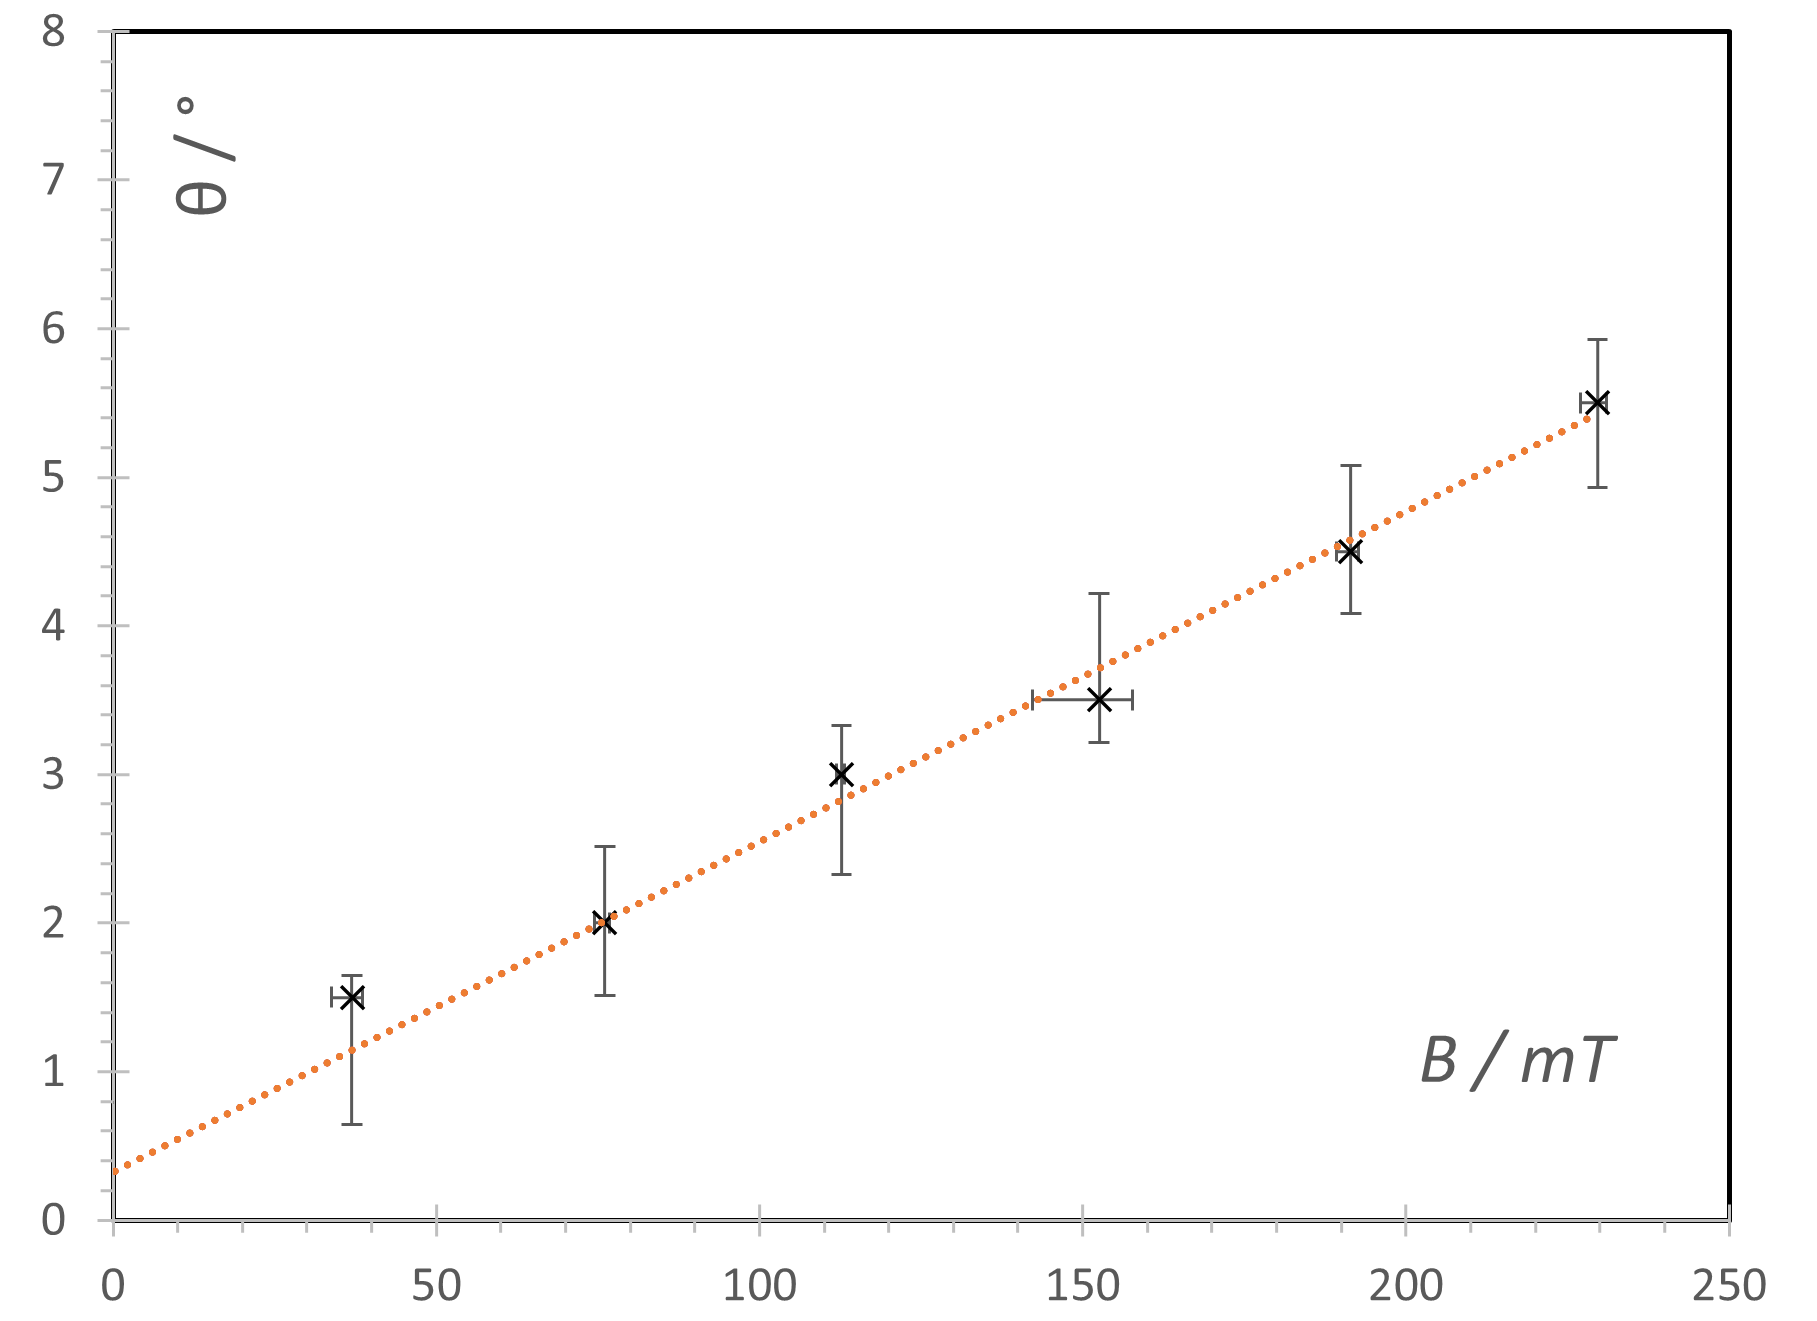
\includegraphics[width=\textwidth, height=200px]{green.png}
        \caption{$\lambda = 515nm$}
        \label{fig:first}
    \end{subfigure}
    \hfill
    \begin{subfigure}{0.475\textwidth}
        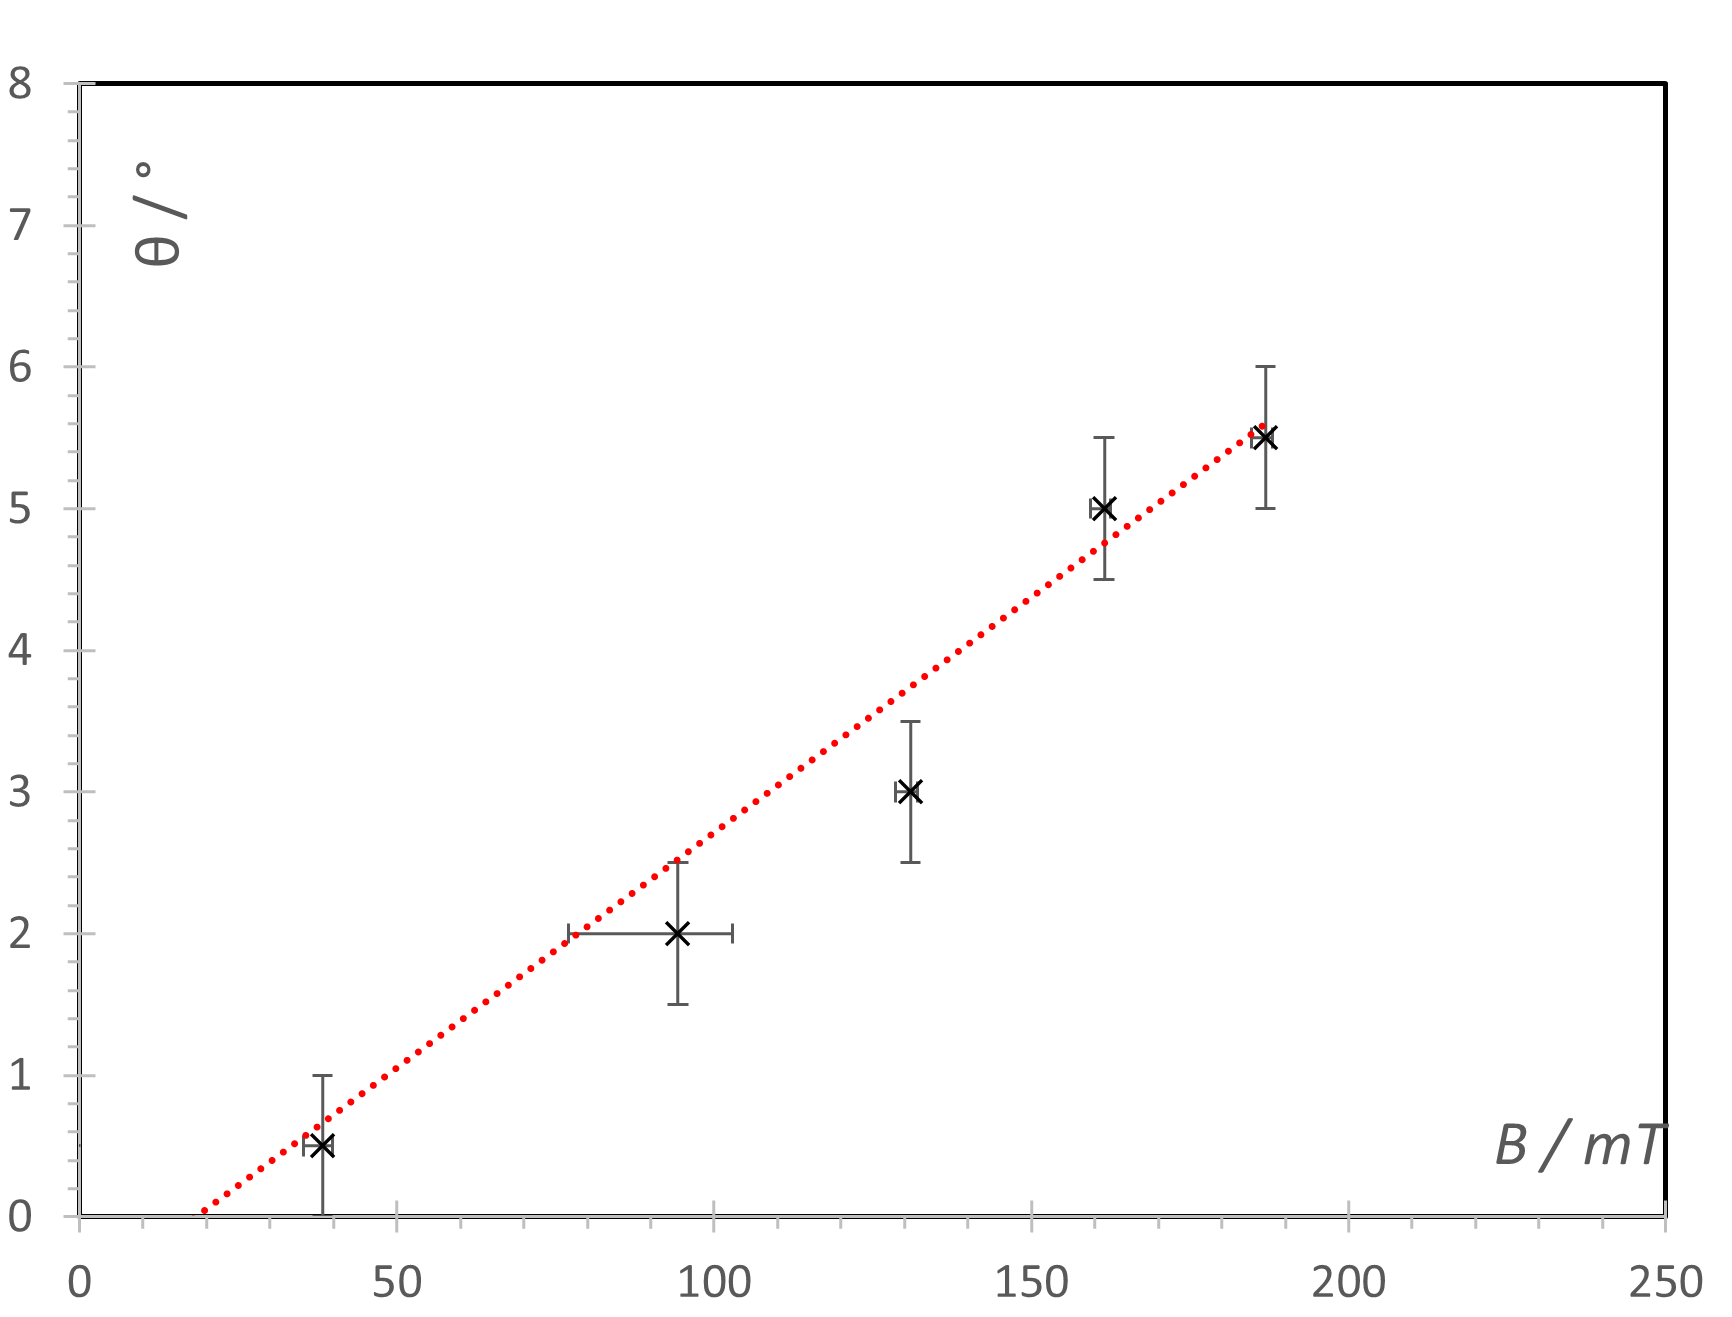
\includegraphics[width=\textwidth, height=200px]{yellow.png}
        \caption{$\lambda = 450nm$}
        \label{fig:second}
    \end{subfigure}
    \hfill
    
    \begin{subfigure}{0.475\textwidth}
        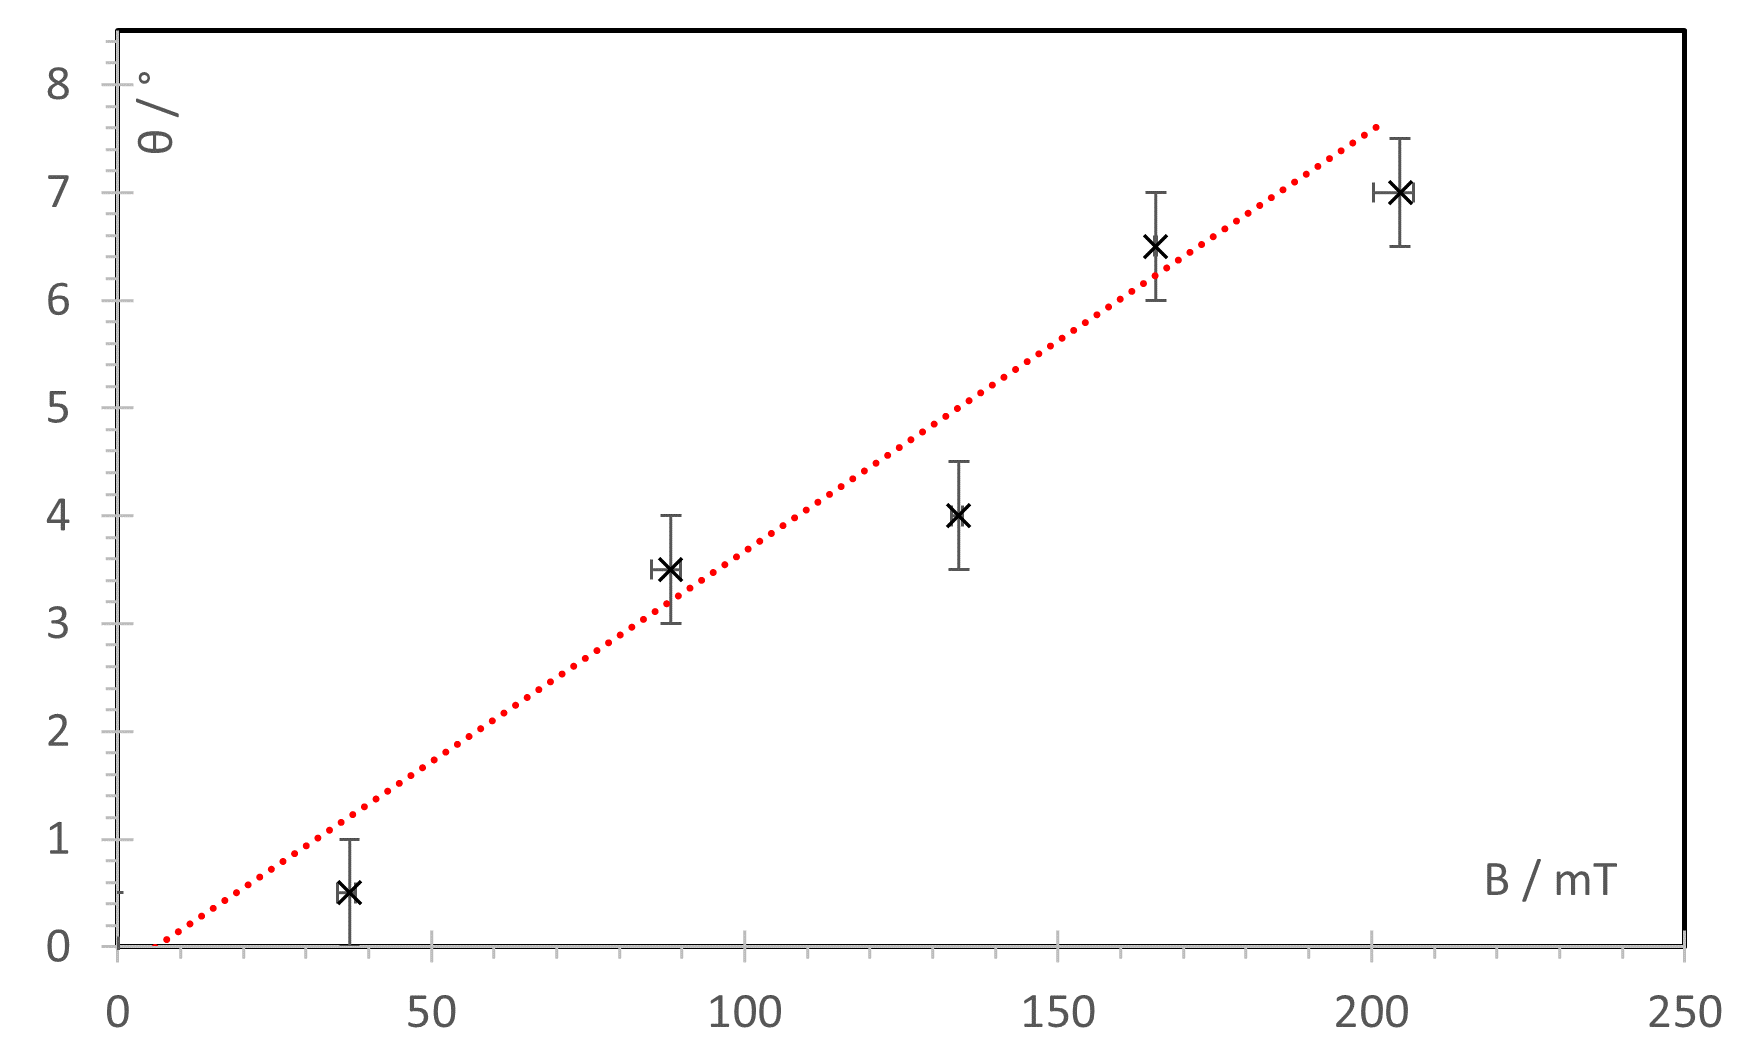
\includegraphics[width=\textwidth, height=200px]{blue.png}
        \caption{$\lambda = 440nm$}
        \label{fig:third}
    \end{subfigure}
    \hfill
    \begin{subfigure}{0.475\textwidth}
        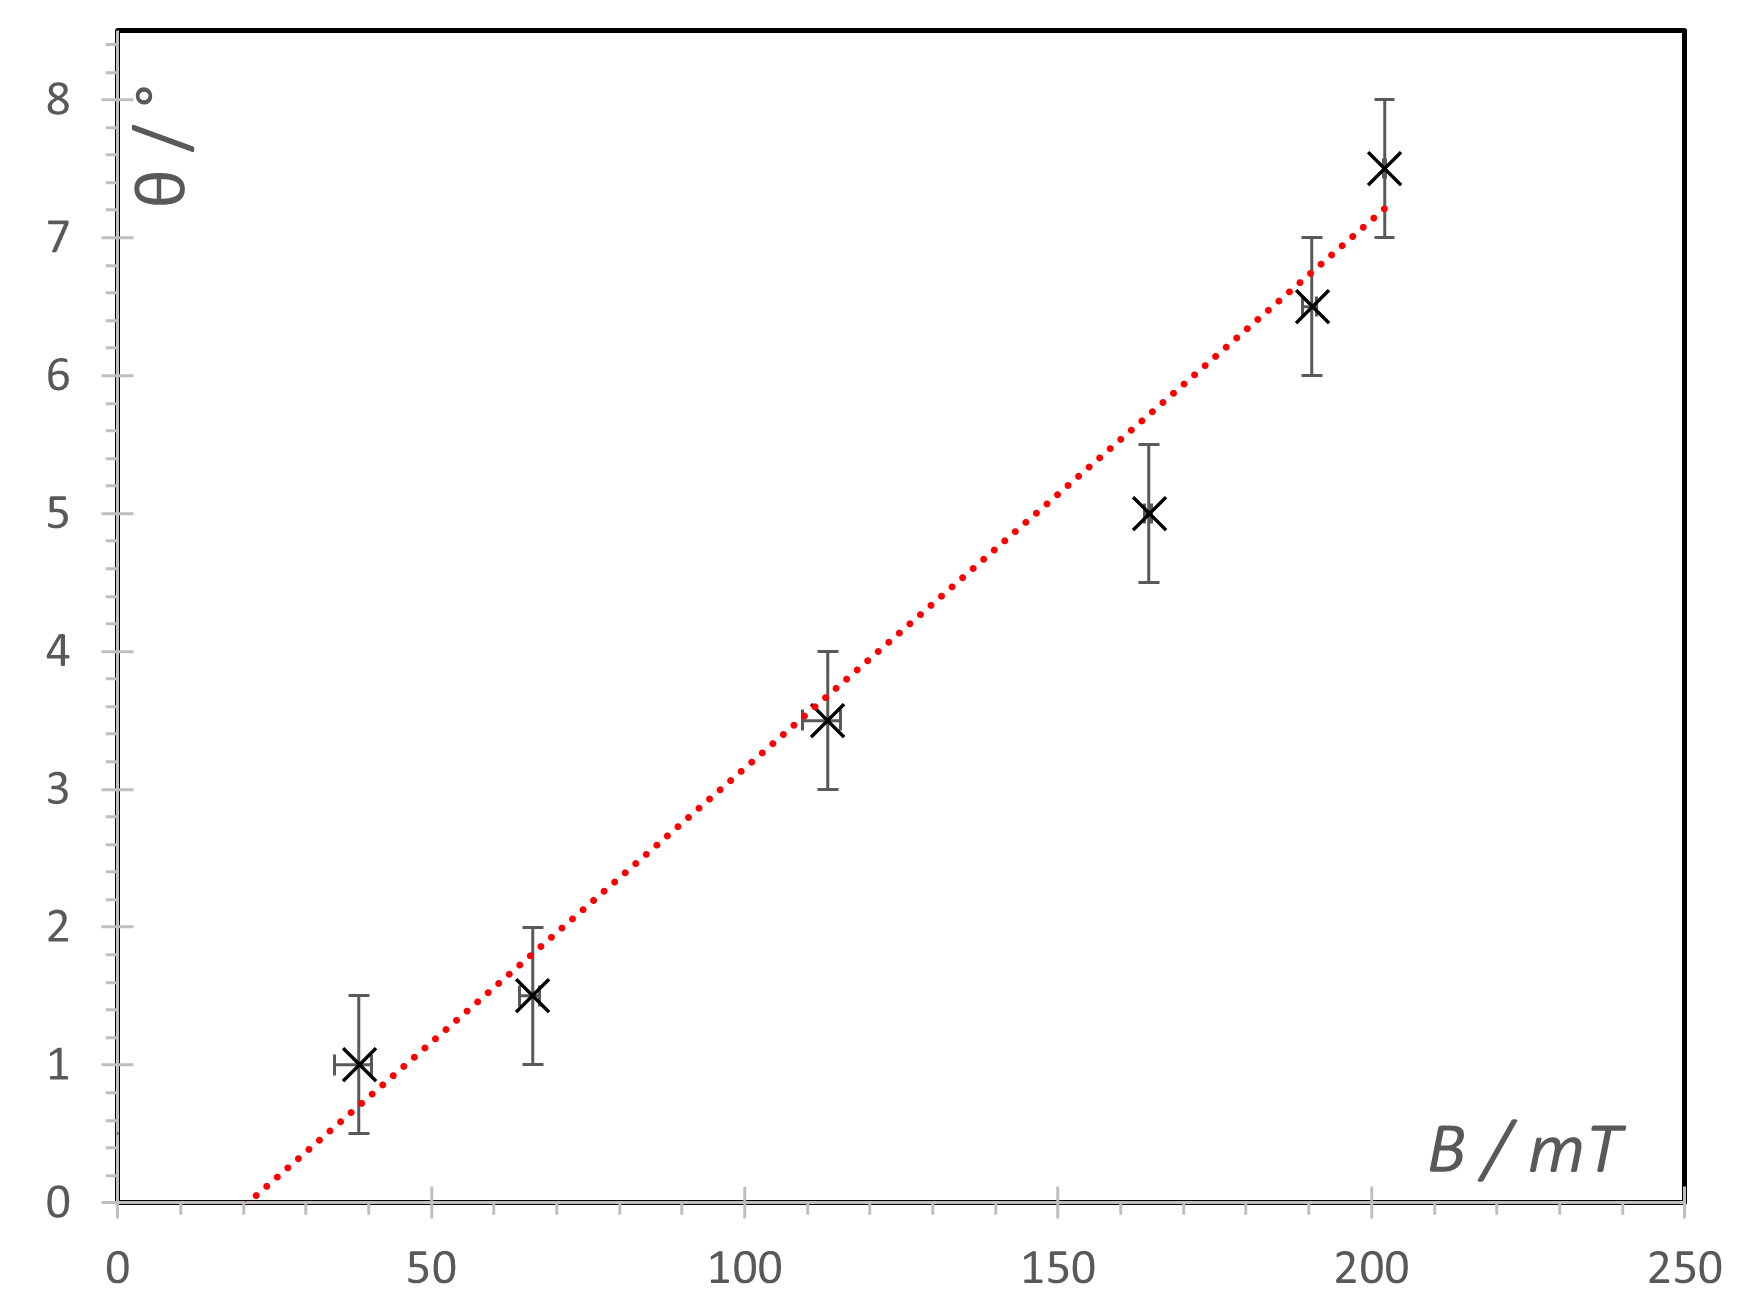
\includegraphics[width=\textwidth, height=200px]{white.png}
        \caption{$\lambda = 570nm$}
        \label{fig:third}
    \end{subfigure}
    \hfill
    \caption{Plot of $\theta$ on B for various wavelengths of incident radiation}
    \label{fig:figures}
\end{figure}

\section{Analysis}
\subsection{Verdet constant - relation to incident wavelength}

Using the values gathered in table 3, it was possible to investigate the relation between the Verdet constant and the incident wavelength. Using the $\chi^{2}$ method iterated over values for possible exponents, x, I found that the best fit with available corresponded to $x = -1.71 \pm 0.90 $.
This is in 'excellent' agreement \cite{HH} with the theoretical value suggested in equation (4). Ploting the $ln(V)$ on $ln(\lambda)$ allows this relation to be visualised.


\begin{figure}[H]%
    \centering%
    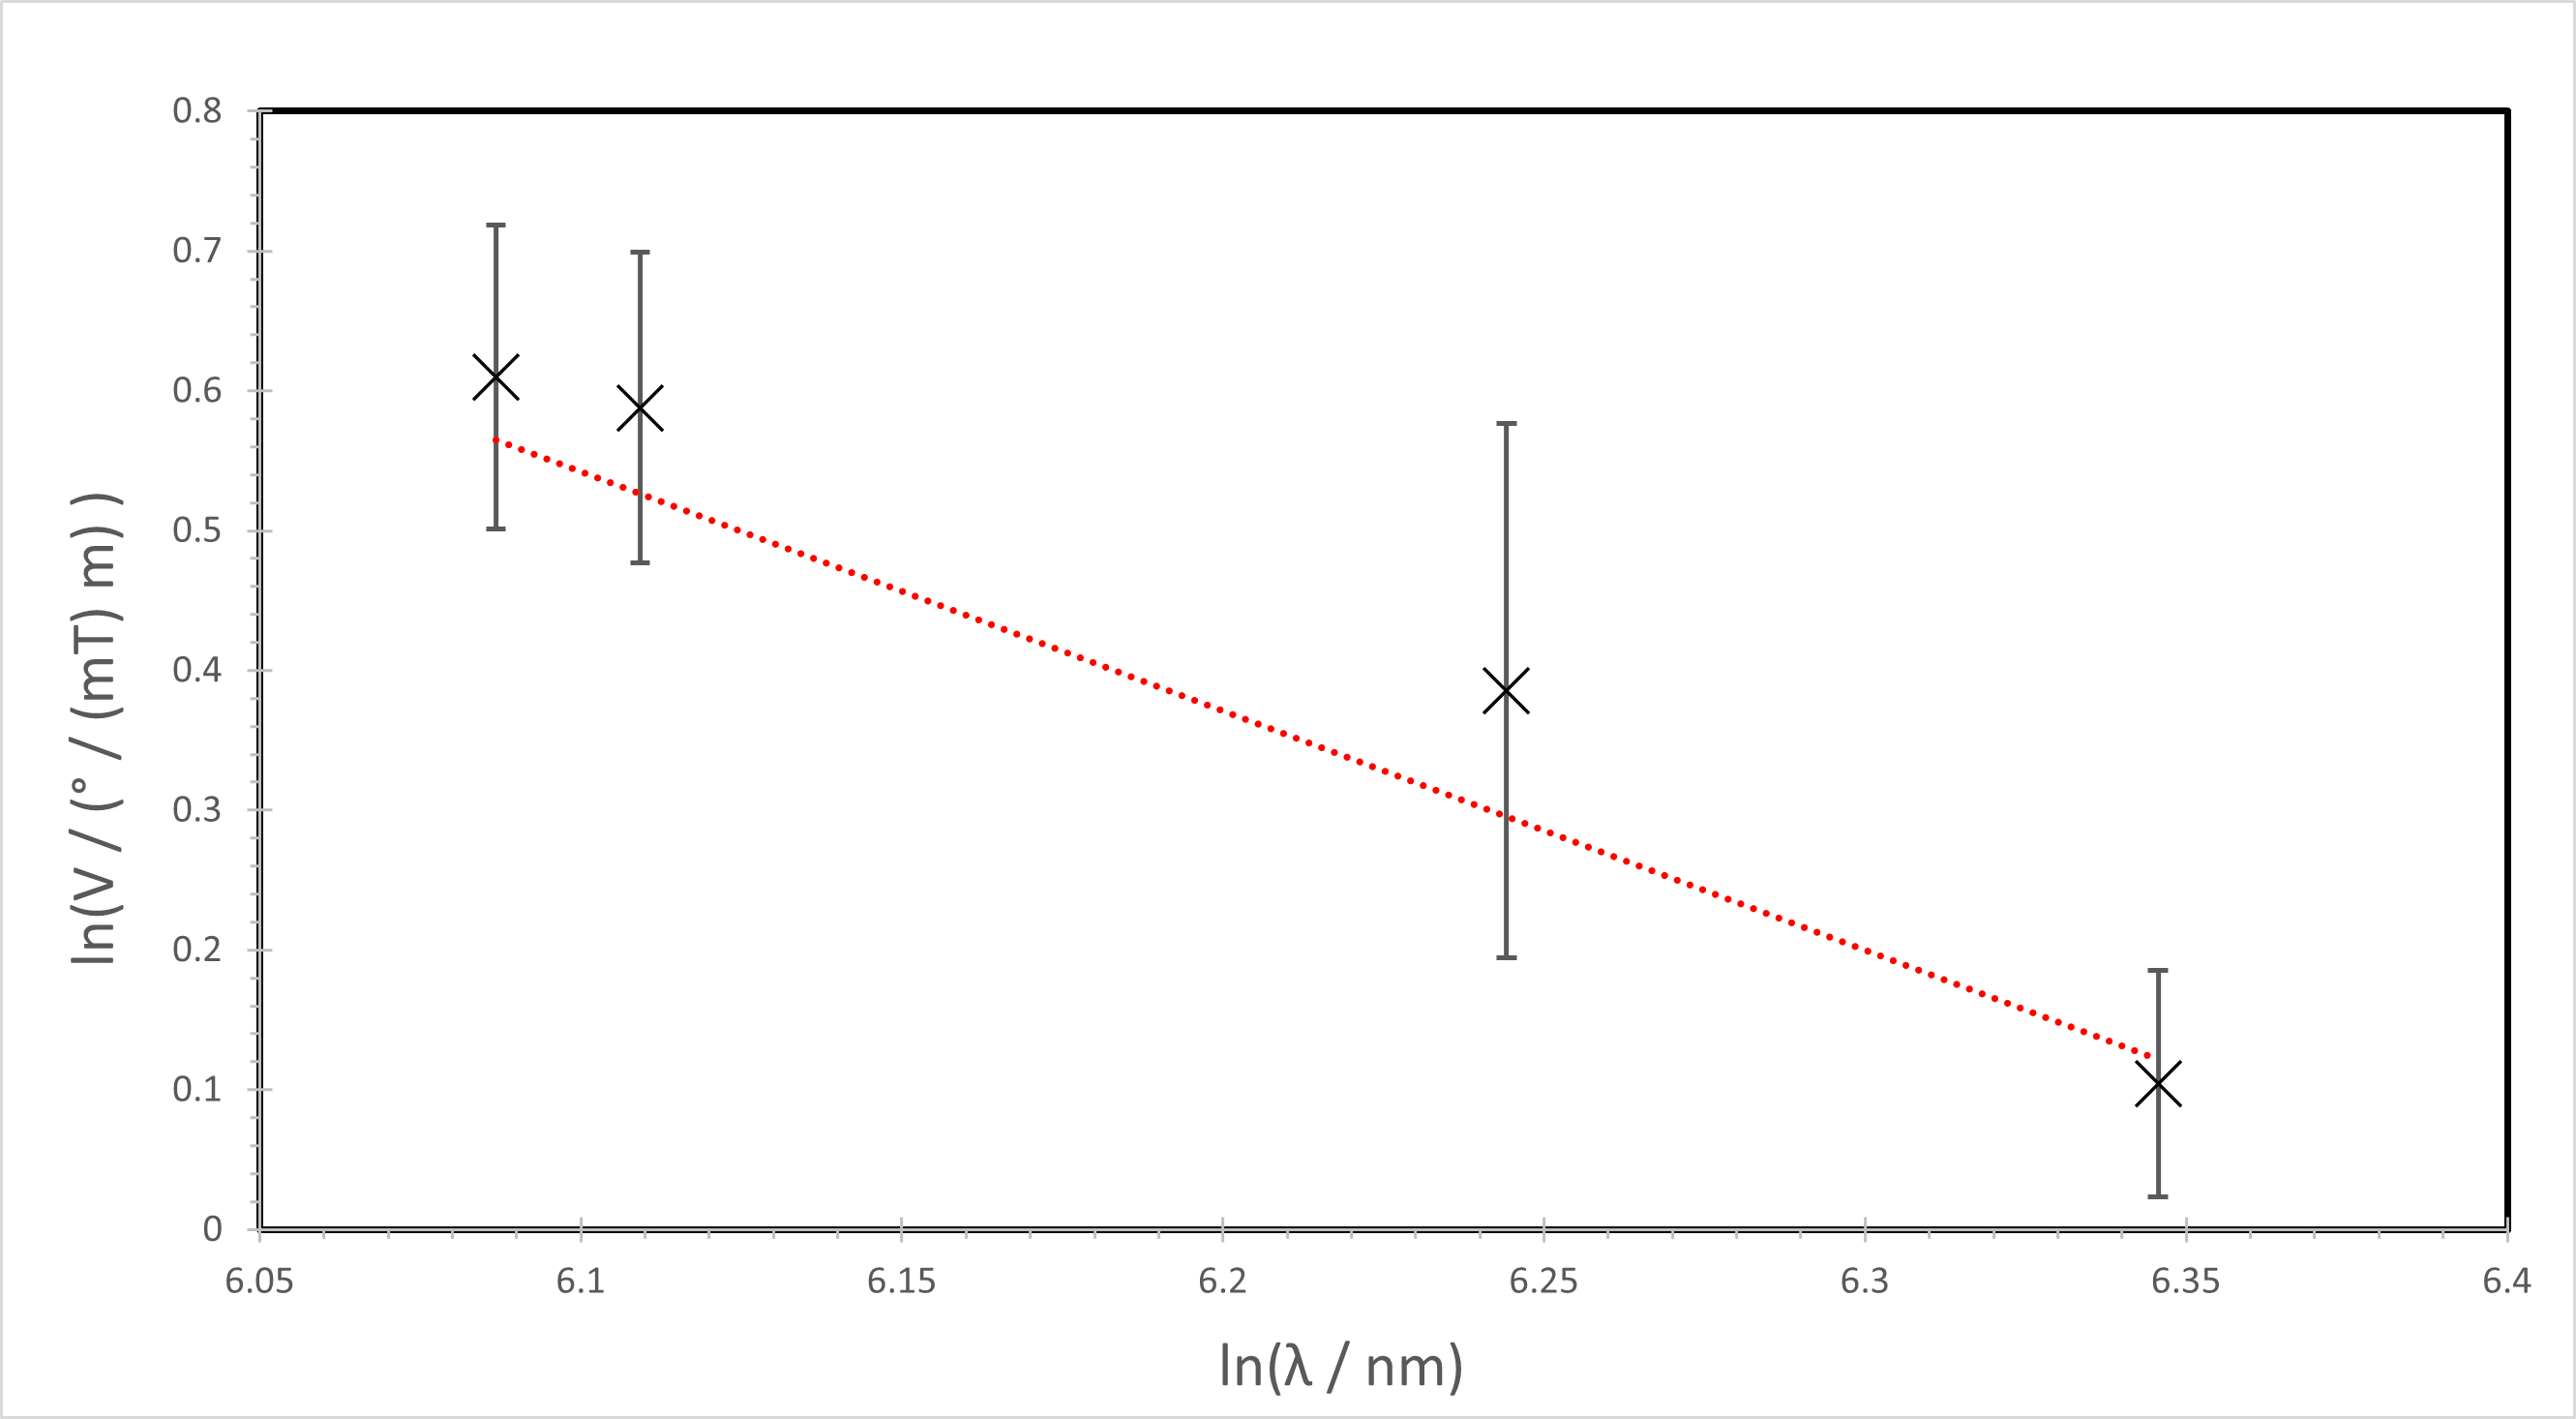
\includegraphics[width=400px]{verdet.png}%
    \caption{$ln(V)$ on $ln(\lambda)$}%
\end{figure}

To compare the measured values for the Verdet constants I plotted data gathered by Kim et. al \cite{Kim} with my fitted data. 
After examing the data more closely, the experimental data showed much more variation than the $\chi^2$ method had led me to believe. For example, the blue filter data ($\lambda=440nm$) gave $V=1.84\pm0.73$ when considering the standard deviation as a measure of error.
It is possible that I have not taken in to account some external uncertainties in my $\chi^{2}$ analysis. Plotting with the more conservative error estimate, we can see at least reasonable agreement that the data lies within at most two standard errors of the literature.

\begin{figure}[H]%
    \centering%
    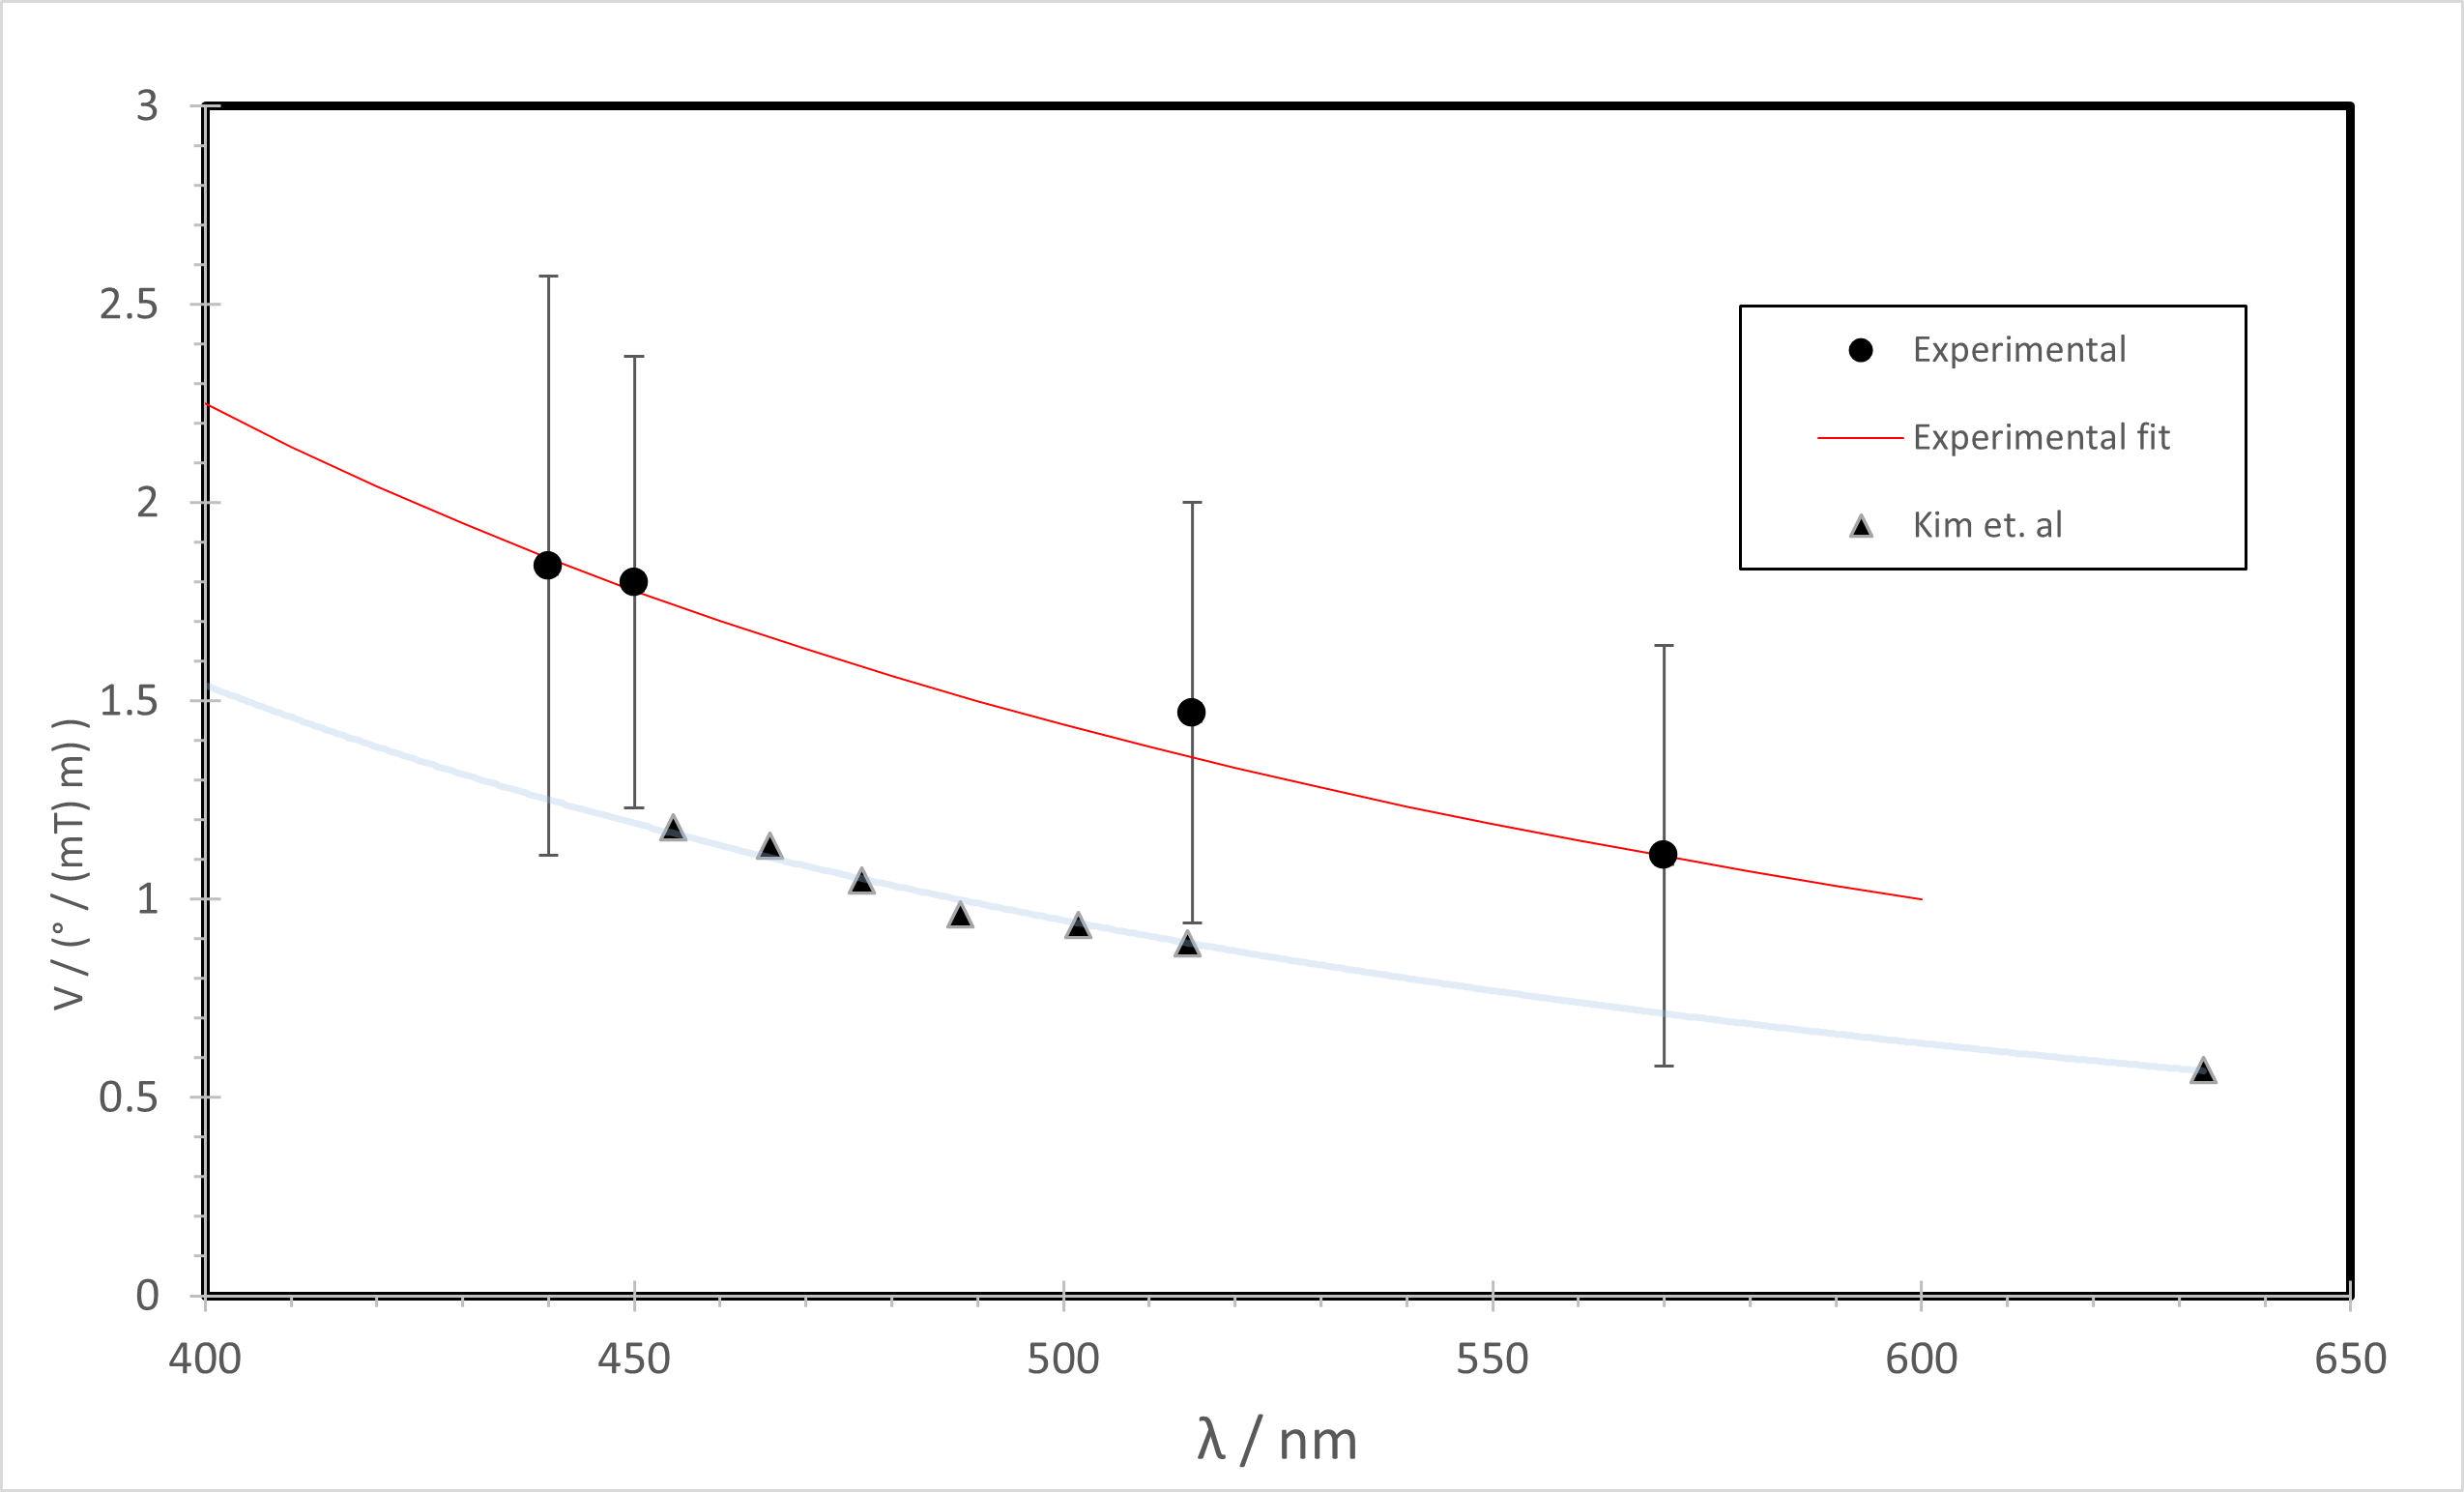
\includegraphics[width=400px]{theoretical.png}%
    \caption{$ln(V)$ on $ln(\lambda)$}%
\end{figure}


However, it is evident that my data shows systemic bias towards higher values for the Verdet constant across the wavelengths in the visible regime. This will need to be addressed.

\subsection{Discussion of the results} 
The results show agreement within the uncertainties, that the Verdet constant follows an inverse square law with the wavelength of incident radiation. However, the values for the Verdet constant are systemically larger compared to the literature values provided by Kim et. al. \cite{Kim}
I believe the primary explaination lies within our experimental method. The assumption that I alluded to earlier, that the current provided to the electromagnet will produce a magnetic field inside the F2 Schott glass according to the calibration curve in figure (1) is flawed.

Firstly, I have not accounted for how the F2 Schott glass behaves when subjected to an external magnetic field. For example, the effect of magnetic hysteresis in the glass is to delay the change of the magnetic field inside the glass, which changes the true magnitude of the field and hence the deflection angle.
My results were taken after testing the equipment and then sequentially taking measurements without demagnetising the iron core or the Schott glass. It is then possible that some residual field exists causing the the cailbration to underestimate the magnetic field, explaining why greater Verdet constants were measured.
However, reversing the polarity of the magnetic fields between measurements should in theory, mitigate this. I could try to use a demagnetising device to ensure that the B field is zero before each measurement to test this hypothesis.

Further the calibration curve figure (1) has not taken into account the effect of heating the electromagnet to high temperatures in short periods and can no longer be considered as linear.
Some evidence can be seen in the increasing magnitdue in the uncertainty of V as we progress through measurements. The heating in the iron core induces errors with the calibration curve. Of course, at high currents the core will heat but I believe this effect was increased by the changing of current directions for each measurement and with the speed in which measurements were taken. 
This is prehaps analogous to the heating effect an iron core experiences under alternating current, which may explain the variabilty of our data expressed with the rather large errors in figure 5. It is important to note that the iron core will also experience the effects of hysteresis, potentially contributing to the effects of the hysteresis hypothesis outlined above. 


Additionally, we have not accounted for uncertainties in the wavelength of the incident radiation. We have assumed that the filter will permit only the wavelength described by the manufacturer and that the source is truly polychromatic containing all the necessary wavelengths. This could be improved by calibrating the filters and estimate the uncertainty in wavelength, prehaps using a CCD and preset software.

\section{Conclusion}

I have verfied the Faraday effect showing that the rotation angle of the polarisation plane is linear with respect to the magnitude of the applied magnetic field.
Furthermore, I have demonstrated agreement with the theoretical prediction of the inverse square relation between the Verdet constant and incident wavelength of radiation. I have compared this measured data with the literature and found limitations with my experimental technique.
Further consideration must be taken with respect to the control and measurement of the magnetic field within the glass.
\printbibliography
\end{document}